% 
% Lecture Template for ME3023 -  Measurements in Mechanical Systems - Tennessee Technological University
%
% Spring 2020 - Summer 2020
% Tristan Hill, May 07, 2020 - June 12, 2020
% Module 4 - Strain Gauges
% Topic 1 - Measuring Strain
%

\documentclass{beamer}                         % for presentation (has nav buttons at bottom)
%\documentclass[handout]{beamer}  % for handout 
\usepackage{beamerthemesplit}
\usepackage{amsmath}
\usepackage{listings}
\usepackage{multicol}
\usepackage{framed}

\beamertemplateballitem

% custom colors
\definecolor{TTUpurple}{rgb}{0.3098, 0.1607, 0.5176} % TTU Purple (primary)
\definecolor{TTUgold}{rgb}{1.0000, 0.8666, 0.0000} % TTU Gold (primary) 
\definecolor{mygray}{rgb}{.6, .6, .6}
\definecolor{mypurple}{rgb}{0.6,0.1961,0.8}
\definecolor{mybrown}{rgb}{0.5451,0.2706,0.0745}
\definecolor{mygreen}{rgb}{0, .39, 0}
\definecolor{mypink}{rgb}{0.9960, 0, 0.9960}

% color commands
\newcommand{\R}{\color{red}}
\newcommand{\B}{\color{blue}}
\newcommand{\BR}{\color{mybrown}}
\newcommand{\K}{\color{black}}
\newcommand{\G}{\color{mygreen}}
\newcommand{\PR}{\color{mypurple}}
\newcommand{\PN}{\color{mypink}}
\newcommand{\OR}{\color{TTU}}
\newcommand{\GD}{\color{TTUgold}}


\setbeamercolor{palette primary}{bg=TTUpurple,fg=TTUgold}
\setbeamercolor{palette secondary}{bg=black,fg=TTUgold}
\setbeamercolor{palette tertiary}{bg=black,fg=TTUpurple}
\setbeamercolor{palette quaternary}{bg=TTUgold,fg=black}
\setbeamercolor{structure}{fg=TTUpurple} % itemize, enumerate, etc
\setbeamercolor{section in toc}{fg=TTUpurple} % TOC sections

%\usefonttheme{professionalfonts}

\newcommand{\Lagr}{\mathcal{L}} % lagrangian

\newcommand{\hspcu}{\underline{\hspace{20mm}}} % large horizontal space w underline
\newcommand{\vspccc}{\vspace{6mm}\\} % large vertical space
\newcommand{\vspcc}{\vspace{4mm}\\}   % medium vertical space
\newcommand{\vspc}{\vspace{2mm}\\}     % small vertical space

\newcommand{\hspcccc}{\hspace{10mm}} % large horizontal space
\newcommand{\hspccc}{\hspace{6mm}} % large horizontal space
\newcommand{\hspcc}{\hspace{4mm}}   % medium horizontal space
\newcommand{\hspc}{\hspace{2mm}}     % small horizontal space

\newcommand{\eqscl}{0.9}     % small horizontal space


\author{ME3023 - Measurements in Mechanical Systems} % original formatting from Mike Renfro, September 21, 2004

\newcommand{\MNUM}{9\hspace{2mm}} % Module number
\newcommand{\TNUM}{1\hspace{2mm}} % Topic number 
\newcommand{\moduletitle}{Strain Gauges}
\newcommand{\topictitle}{Measuring Strain} 

\newcommand{\sectiontitleI}{Motivation in Design}
\newcommand{\sectiontitleII}{Stress and Strain}
\newcommand{\sectiontitleIII}{The Strain Gauge}
\newcommand{\sectiontitleIV}{Engineering Applications}

% custom box
\newsavebox{\mybox}

\title{Module \MNUM - \moduletitle}

\date{Mechanical Engineering\vspc Tennessee Technological University}

\begin{document}

\lstset{language=MATLAB,basicstyle=\ttfamily\small,showstringspaces=false}

\frame{\titlepage \center\begin{framed}\Large \textbf{Topic \TNUM - \topictitle}\end{framed} \vspace{5mm}}

% Section 0: Outline
\frame{

\large \textbf{Topic \TNUM - \topictitle} \vspace{3mm}\\

\begin{itemize}

	\item \sectiontitleI		\vspc % Section I
	\item \sectiontitleII 	\vspc % Section II
	\item \sectiontitleIII 	\vspc %Section III
	\item \sectiontitleIV 	\vspc %Section IV

\end{itemize}

}

% Section I:
\section{\sectiontitleI}

% Section I - Frame I:
\frame{
\frametitle{\sectiontitleI}

The design of load-carrying components for machines and structures requires information concerning the {\B distribution of forces within the particular component}. Proper design of devices such as shafts, pressure vessels, and support structures must consider {\PR load-carrying capacity and allowable deflections}. Mechanics of materials provides a basis for predicting these essential characteristics of a mechanical design, and provides the fundamental understanding of the behavior of load-carrying parts. However, theoretical analysis is often not sufficient, and {\PN experimental measurements} are required to achieve a final design.

{\tiny Text: Theory and Design of Mechanical Measurements}
}


% Section II:
\section{\sectiontitleII}

% Section II - Frame I:
\frame{
\frametitle{\sectiontitleII}

Consider a member under uni-axial loading. The {\R strain} is defined as the ratio of the change in length to the original length of the  component.  

\begin{multicols}{2}
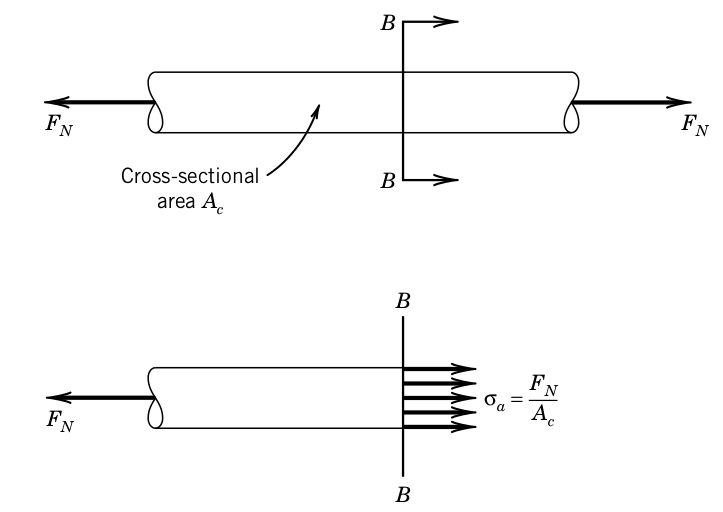
\includegraphics[scale=.25]{strain_fig1.png}


\hspace{15mm}\scalebox{1}{$\sigma_a=\frac{F_N}{A_c}$}\vspace{10mm}\\
\hspace{15mm}\scalebox{1}{$\epsilon_a=\frac{\delta_L}{L}$}\vspace{10mm} \\
\hspace{15mm}\scalebox{1}{$\sigma_a=E_m\epsilon_a$}\vspc
\end{multicols}

}

% Section II - Frame II:
\frame{
\frametitle{\sectiontitleII}

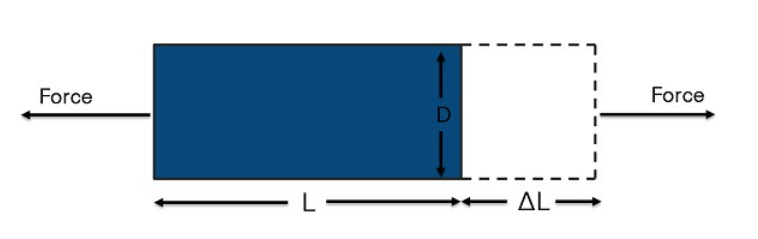
\includegraphics[scale=.20]{strain_fig2.png} 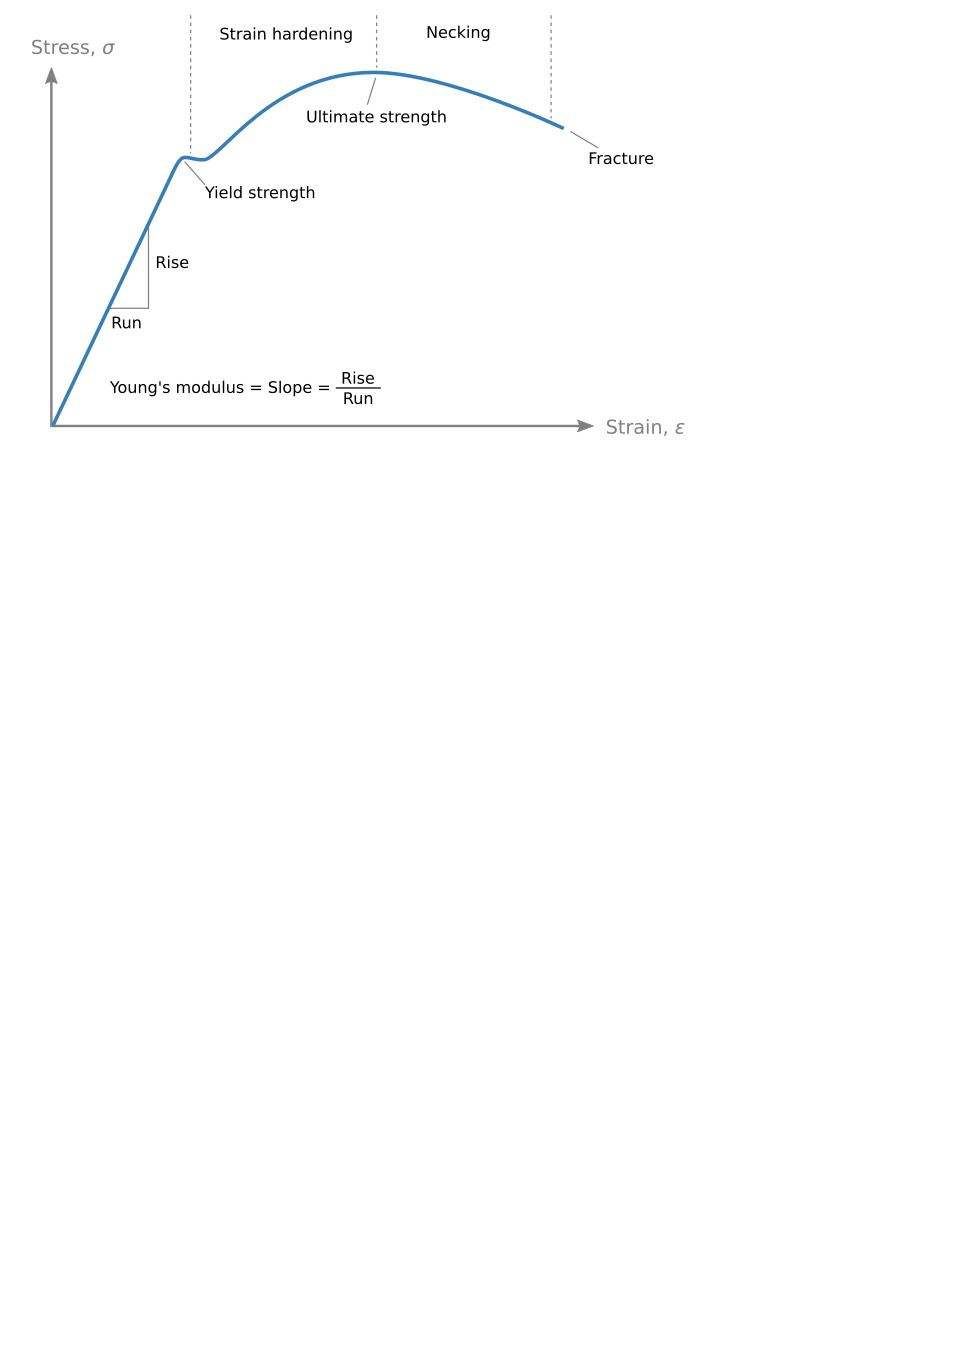
\includegraphics[scale=.5]{stress_strain_fig1.png} 
{\tiny Image: \href{https://commons.wikimedia.org/wiki/File:Stress_strain_ductile.svg}{Wikimedia} }



}


% Section III:
\section{\sectiontitleIII}

% Section I - Frame III:
\frame{
\frametitle{\sectiontitleIII}

... the ideal sensor for the measurement of strain would (1) have good spatial resolution, implying
that the sensor would measure strain at a point; (2) be unaffected by changes in ambient conditions;
and (3) have a high-frequency response for dynamic (time-resolved) strain measurements. A sensor
that closely meets these characteristics is the {\B bonded resistance strain gauge}. \vspc

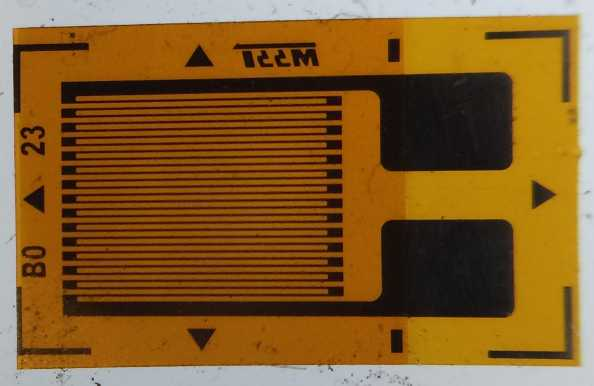
\includegraphics[scale=.20]{unmounted_strain_gauge.jpg}\hspccc 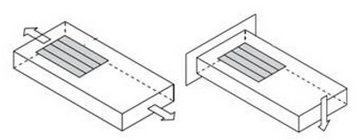
\includegraphics[scale=.4]{mounted_gages.png}

\vspace{20mm}
{\tiny Text: Theory and Design of Mechanical Measurements}
}

% Section I - Frame III:
\frame{
\frametitle{\sectiontitleIII}

Strain gauges can be mounted in different ways for different purposes. We will begin with a single gauge mounted in the axial direction. \vspc

 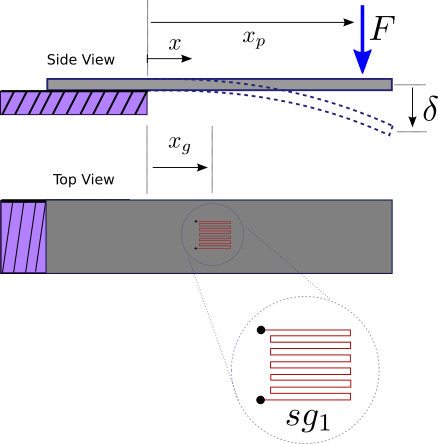
\includegraphics[scale=.4]{axial_gaged_beam.png}

\vspace{20mm}
{\tiny Text: Theory and Design of Mechanical Measurements}
}

% Section IV:
\section{\sectiontitleIV}

% Section I - Frame IV:
\frame{
\frametitle{\sectiontitleIV}

\begin{itemize}



\item Segway back to {\it Motivation in Design} (Slide 1) ... \vspc

\item Aerospace \vspc

\item Infrastructure \vspc

\item Please read this article \href{https://medium.com/@encardio/strain-gauge-principle-types-features-and-applications-357f6fed86a5}{here}. We will cover the mathematics and theory in class but this article has a short section on applications of strain gauges that I want you to see. 

\end{itemize}


}
	
\end{document}





